 \documentclass[letterpaper,11pt]{article}
\usepackage[margin=2cm]{geometry}

\usepackage{graphicx}
\usepackage{amsmath}
\usepackage{amsfonts}
\usepackage{amssymb}
\usepackage{multicol}
\usepackage{listings}

\DeclareMathOperator*{\argmin}{arg\,min}
\DeclareMathOperator*{\argmax}{arg\,max}


\title{\textbf{Pattern Recognition Theory 18794 Homework 1}}
\author{Mengwen He (Alex)}
\date{September 25, 2016}

\begin{document}
\maketitle

\section*{Problem 1}

\begin{enumerate}
\item A vector can be broken up into its direction and magnitude. The equation
$A\vec{v} = \vec{w}$ can seen as applying a linear transformation to vector $\vec{v}$ to get a
different vector $\vec{w}$. If $\vec{v}$ happens to be an eigenvector of A, describe what
happens to the direction of $\vec{v}$ after transformation?\\
\textbf{Answer:}\\
$\because$ $\vec{v}$ is an eigenvector of $A$\\
$\therefore$ $A \vec{v} = \lambda \vec{v}$\\
If the eigenvalue $\lambda > 0$, then the direction of $\vec{v}$ will not change.\\
If the eigenvalue $\lambda < 0$, then the direction of $\vec{v}$ will be inversed.\\
If the eigenvalue $\lambda = 0$, then the direction of $\vec{v}$ will to be an arbitrary direction (definition of the zero vector).

\item Given\\
\begin{equation}
\nonumber
A=\left[\begin{array}{ccc}
1 & 2 & 1 \\
2 & 4 & 2 \\
3 & 3 & 3 \\
\end{array}\right],~
B=\left[\begin{array}{cc}
-1 & 2 \\
2 & 2 \\
\end{array}\right],~
C=\left[\begin{array}{cccc}
2 & 8 & 1 & 0 \\
3 & 12 & 2 & 0 \\
2 & 8 & 3 & -1 \\
\end{array}\right],~
D=\left[\begin{array}{cccc}
2 & 8 & 1 & 1 \\
3 & 12 & 2 & 1 \\
2 & 8 & 3 & -1 \\
\end{array}\right]
\end{equation}
\begin{enumerate}
	\item What is the rank of each matrix?\\
	\textbf{Answer:}
	\begin{itemize}
		\item For the square matrix $A$:
		$$|A - \lambda I|=0 \Rightarrow \lambda^3 - 8 \lambda^2 + 6\lambda = 0 \Rightarrow \left\{\begin{array}{rcl}
		\lambda_1 & = & 4+\sqrt{10} \\
		\lambda_2 & = & 4-\sqrt{10} \\
		\lambda_3 & = & 0 \\
		\end{array}\right. \Rightarrow rank(A)=2$$
		\item For the square matrix $B$:
		$$|B - \lambda I|=0 \Rightarrow \lambda^2 - \lambda - 6 = 0 \Rightarrow
		\left\{\begin{array}{rcl}
		\lambda_1 & = & 3 \\
		\lambda_2 & = & -2 \\
		\end{array}\right. \Rightarrow rank(B)=2$$
		\item For the ``fat" matrix $C$:
		$$\left[\begin{array}{cccc}
		2 & 8 & 1 & 0 \\
		3 & 12 & 2 & 0 \\
		2 & 8 & 3 & -1 \\
		\end{array}\right] \xrightarrow{\begin{array}{c}
		R_2=R_2-\frac{3}{2}R_1 \\
		R_3=R_3-R_1\\
		\end{array}} \left[\begin{array}{cccc}
		2 & 8 & 1 & 0 \\
		0 & 0 & \frac{1}{2} & 0 \\
		0 & 0 & 2 & -1 \\
		\end{array}\right] $$
		$$\xrightarrow{\begin{array}{c}
		R_3 = R_3 - 4 R_2 \\
		\end{array}} \left[\begin{array}{cccc}
		2 & 8 & 1 & 0 \\
		0 & 0 & \frac{1}{2} & 0 \\
		0 & 0 & 0 & -1 \\
		\end{array}\right] \Rightarrow rank(C)=3$$
		\item For the ``fat" matrix $D$:
		$$\left[\begin{array}{cccc}
		2 & 8 & 1 & 1 \\
		3 & 12 & 2 & 1 \\
		2 & 8 & 3 & -1 \\
		\end{array}\right] \xrightarrow{\begin{array}{c}
		R_2=R_2-\frac{3}{2}R_1 \\
		R_3=R_3-R_1\\
		\end{array}} \left[\begin{array}{cccc}
		2 & 8 & 1 & 1 \\
		0 & 0 & \frac{1}{2} & -\frac{1}{2} \\
		0 & 0 & 2 & -2 \\
		\end{array}\right] $$
		$$\xrightarrow{\begin{array}{c}
		R_3 = R_3 - 4 R_2 \\
		\end{array}} \left[\begin{array}{cccc}
		2 & 8 & 1 & 1 \\
		0 & 0 & \frac{1}{2} & -\frac{1}{2} \\
		0 & 0 & 0 & 0 \\
		\end{array}\right] \Rightarrow rank(D)=2$$
	\end{itemize}
	
	\item What is the trace of each matrix?\\
	\textbf{Answer:}
	\begin{itemize}
		\item For square matrix $A$: $trace(A)=1+4+3=(4+\sqrt{10})+(4-\sqrt{10})+0=8$
		\item For square matrix $B$: $trace(B)=-1+2=3+(-2)=1$
		\item For ``fat" matrices $C$ and $D$: trace is only defined for square matrix.
	\end{itemize}
	\item What is the determinant of matrices $A$, $B$?\\
	\textbf{Answer:}
	\begin{itemize}
		\item For matrix $A$: $det(A)=(4+\sqrt{10})*(4-\sqrt{10})*0=0$
		\item For matrix $B$: $det(B)=3*(-2)=-6$
	\end{itemize}
	\item Find the eigenvalues and eigenvectors of $B$.\\
	\textbf{Answer:}\\
	From 2.(a), $B$'s eigenvalues are $\lambda_1=3,~\lambda_2=-2$\\
	Assume $B$'s eigenvectors are $\vec{v}_1=[v_{11},v_{12}]^T (v_{11} \geq 0),~\vec{v}_2=[v_{21},v_{22}]^T (v_{21} \geq 0)$
	$$\left[\begin{array}{cc}
	-1 & 2 \\
	2 & 2 \\
	\end{array}\right] \left[\begin{array}{cc}
	v_{11} & v_{21} \\
	v_{12} & v_{22} \\
	\end{array}\right] = \left[\begin{array}{cc}
	v_{11} & v_{21} \\
	v_{12} & v_{22} \\
	\end{array}\right] \left[\begin{array}{cc}
	\lambda_1 & 0 \\
	0 & \lambda_2 \\
	\end{array}\right] \Rightarrow \left\{\begin{array}{c}
	2v_{11}-v_{12}=0 \\
	v_{21}+2v_{22}=0 \\
	v_{11}^2+v_{12}^2=1 \\
	v_{21}^2+v_{22}^2=1 \\
	\end{array}\right. \Rightarrow \left\{\begin{array}{c}
	v_{11}=\frac{\sqrt{5}}{5} \\
	v_{12}=\frac{2\sqrt{5}}{5} \\
	v_{21}=\frac{\sqrt{5}}{5} \\
	v_{22}=-\frac{2\sqrt{5}}{5} \\
	\end{array}\right.$$
	Therefore $B$'s eigenvector are $\vec{v}_1=\left[\frac{\sqrt(5)}{5},\frac{2\sqrt{5}}{5}\right]^T ,~\vec{v}_2=\left[\frac{\sqrt(5)}{5},-\frac{2\sqrt{5}}{5}\right]^T$
	\item What is the dimension of the null space of each of the matrices?\\
	\textbf{Answer:}
	\begin{itemize}
		\item For the matrix $A$: $dim(Null(A))=dim(A)-rank(A)=3-2=1$
		\item For the matrix $B$: $dim(Null(B))=dim(B)-rank(B)=2-2=0$
		\item For the matrix $C$:
		\begin{itemize}
			\item Right null space: $dim(Null(C))=col\_dim(C)-rank(C)=4-3=1$
			\item Left null space: $dim(Null(C^T))=col\_dim(C^T)-rank(C^T)=3-3=0$
		\end{itemize}
		\item For the matrix $D$:
		\begin{itemize}
			\item Right null space: $dim(Null(D))=col\_dim(D)-rank(D)=4-2=2$
			\item Left null space: $dim(Null(D^T))=col\_dim(D^T)-rank(D^T)=3-2=1$
		\end{itemize}
	\end{itemize}
\end{enumerate}
\end{enumerate}

\newpage

\section*{Problem 2}

\begin{enumerate}
\item Prove that if $P$ is an orthogonal matrix, then $PP^T$ is a projection matrix.\\
\textbf{Answer:}
\begin{enumerate}
\item Method 1:\\
$\because P$ is an orthogonal matrix\\
$\therefore PP^T=I$\\
$\therefore PP^T$ is a projection matrix.
\item Method 2:\\
$\because P$ is an orthogonal matrix\\
$\therefore (PP^T)(PP^T)=P(P^TP)P^T=PP^T$\\
$\therefore PP^T$ is a projection matrix.
\end{enumerate}

\item Under what condition(s), for arbitrary non-zero matrices $A,B \in \mathbb{R}^{m \times n}$, do we have $rank(A + B) = rank(A) + rank(B)$? (Hint: Think singular values/vectors)\\
\textbf{Answer:}\\
$\because$ $dim(colsp([A,B]))=dim(colsp(A))+dim(colsp(B))-dim(colsp(A) \bigcap colsp(B))$\\
$\therefore$ $dim(colsp([A,B]))=rank(A)+rank(B)-dim(colsp(A) \bigcap colsp(B))$\\
$\because$ $colsp(A+B)$ is a subspace of $colsp([A,B])$\\
$\therefore$ $dim(colsp([A,B])) \geq dim(colsp(A+B)) = rank(A+B)$\\
$\therefore$ $rank(A)+rank(B) \geq rank(A+B) + dim(colsp(A) \bigcap colsp(B))$\\
If we have $rank(A+B)=rank(A)+rank(B)$,\\
then $dim(colsp(A) \bigcap colsp(B))=0 \Rightarrow colsp(A) \bigcap colsp(B)=\{\vec{0}\} \Rightarrow A^TB=0$\\
Therefore, we get a necessary condition as below:\\
For all matrices $A,B \in \mathbb{R}^{m \times n}$, $rank(A+B)=rank(A)+rank(B)$ $\Rightarrow$ $A^TB=0$.\\
So, if under $colsp(A) \bigcap colsp(B)=\{\vec{0}\}$ (strong) or $A^TB=0$ (weak), for all matrices $A,B \in \mathbb{R}^{m \times n}$, we can have $rank(A+B)=rank(A)+rank(B)$.

\item In general, does a relation exist between the rank of a sum of matrices and the sum of the ranks of the individual matrices?\\
\textbf{Answer:}\\
To find the relationship between $rank(\sum_{i=1}^{N}{A_i})$ and $\sum_{i=1}^{N}{rank(A_i)}$\\
From 2, we know that $rank(A+B) \leq rank(A)+rank(B)-dim(colsp(A) \bigcap colsp(B))$\\
Therefore, we gradually derive that relationship as below:\\
$rank(\sum_{i=1}^{N}{A_i}) \\
\leq rank(A_1) + rank(\sum_{i=2}^{N}{A_i}) - dim(colsp(A_1) \bigcap colsp(\sum_{i=2}^{N}{A_i}))$\\
$\leq rank(A_1) + rank(A_2) + rank(\sum_{i=3}^{N}{A_i}) - dim(colsp(A_2) \bigcap colsp(\sum_{i=3}^{N}{A_i})))$\\
$...$\\
$\leq \sum_{i=1}^{N}{rank(A_i)}$

\item Under the premise of problem 1.2, you arrived at a condition. Is the condition sufficient to ensure that $\sigma_{max} (A+B) = max (\sigma_{max} (A), \sigma_{max}(B))$? If not, what else do you need to constrain ? Here, $\sigma_{max} (A)$ is the maximum singular value of $A$\\
\textbf{Answer:}\\
$\because$ From the definition of matrix LSV-norm: $$||A||_2=\max_{\vec{x}:||\vec{x}||_2=1}{||A\vec{x}||_2}=\sigma_{max}(A)$$
$\therefore$ $$\sigma_{max}(A+B)=\max_{\vec{x}:||\vec{x}||_2=1}{||(A+B)\vec{x}||_2}$$
$\therefore$ $$\sigma_{max}^2(A+B)=\max_{\vec{x}:||\vec{x}||_2=1}{((A+B)\vec{x})^T((A+B)\vec{x})}$$
$$\sigma_{max}^2(A+B)=\max_{\vec{x}:||\vec{x}||_2=1}{((A\vec{x})^TA\vec{x}+(B\vec{x})^TB\vec{x}+2\vec{x}^T(A^TB)\vec{x})}$$
$\because$ we are under the condition $rank(A+B)=rank(A)+rank(B) \Rightarrow A^TB=0$ given by 2\\
$\therefore$ $$\sigma_{max}^2(A+B)=\max_{\vec{x}:||\vec{x}||_2=1}{((A\vec{x})^TA\vec{x}+(B\vec{x})^TB\vec{x})}$$
$$\sigma_{max}^2(A+B)=\max_{\vec{x}:||\vec{x}||_2=1}{(||A\vec{x}||_2^2+||B\vec{x}||_2^2)}$$
Assume:
$$\vec{x}_A^*=\argmax_{\vec{x}:||\vec{x}||_2=1}{||A\vec{x}||_2}$$
$$\vec{x}_B^*=\argmax_{\vec{x}:||\vec{x}||_2=1}{||B\vec{x}||_2}$$
$$\vec{x}^*=\argmax_{\vec{x}:||\vec{x}||_2=1}{||(A+B)\vec{x}||_2}$$

\begin{itemize}
\item If $\vec{x}^* = \vec{x}_A^*$, then $\sigma_{max}(A+B) = \sqrt{\sigma_{max}^2(A) + ||B\vec{x}_A^*||_2^2 } \geq \sigma_{max}(A)$
\item If $\vec{x}^* = \vec{x}_B^*$, then $\sigma_{max}(A+B) = \sqrt{||A\vec{x}_B^*||_2^2 + \sigma_{max}^2(B)} \geq \sigma_{max}(B)$
\end{itemize}
$\therefore$ with the condition $rank(A+B)=rank(A)+rank(B)$, we derived that $\sigma_{max}(A+B) \geq max (\sigma_{max} (A), \sigma_{max}(B))$\\
$\therefore$ $rank(A+B)=rank(A)+rank(B) \not \Rightarrow \sigma_{max}(A+B) = max (\sigma_{max} (A), \sigma_{max}(B))$ (it is not a sufficient condition)\\
However, we can add another condition that $rowsp(A) \bigcap rowsp(B) = \{\vec{0}\} \Rightarrow AB^T=0$\\
First we can guarantee that:
\begin{itemize}
\item If $\vec{x}^* = \vec{x}_A^* \in rowsp(A)$, then $\sigma_{max}(A+B) = \sqrt{\sigma_{max}^2(A) + ||B\vec{x}_A^*||_2^2 } = \sigma_{max}(A)$
\item If $\vec{x}^* = \vec{x}_B^* \in rowsp(B)$, then $\sigma_{max}(A+B) = \sqrt{||A\vec{x}_B^*||_2^2 + \sigma_{max}^2(B)} = \sigma_{max}(B)$
\end{itemize}
Then, we need to demonstrate that:
$$\forall\text{ unit }\vec{x} \in \mathbb{R}^m, \sqrt{||A\vec{x}||_2^2 + ||B\vec{x}||_2^2} \leq max(\sigma_{max}(A),\sigma_{max}(B))$$
Do SVD decomposition on any matrix $M \in \mathbb{R}^{n \times m}$: $M=U_MS_MV_M^T$\\
$\because$ For $M\vec{x}=U_MS_MV_M^T\vec{x}$, the unit $\vec{x}$ is first projected into $rowsp(V_M)$ by $V_M$, then scaled by $S_M$ along the bases in $rowsp(V_M)$, and finally projected into $colsp(U_M)$ (but actually into $colsp(M)$) by $U_M$.\\
So we define a $\hat{S}_M$ from $S_M$ as below:
$$\hat{S}_M^{ij}=\left\{\begin{array}{cl}
1, & S_M^{ij} \neq 0 \\
0, & S_M^{ij} = 0 \\
\end{array}\right.$$
And we define the energy projected into $colsp(A)$ from unit $\vec{x}$ by using $U_M\hat{S}_MV_M^T$ as $$E_M(\vec{x})=||U_M\hat{S}_MV_M^T\vec{x}||_2^2$$
By definition, we know that (assume $rowsp(A) \bigcap rowsp(B)=\{\vec{0}\}$):
\begin{itemize}
\item If unit $\vec{x} \in rowsp(A)$, then $E_A(\vec{x})=1$
\item If unit $\vec{x} \not \in rowsp(A)$, then $E_A(\vec{x})<1$
\item If unit $\vec{x} \in rowsp(B)$, then $E_A(\vec{x})=0$
\item If unit $\vec{x} \in rowsp([A,B])$, then $E_A(\vec{x})+E_B(\vec{x})=1$
\item If unit $\vec{x} \not \in rowsp([A,B])$, then $E_A(\vec{x})+E_B(\vec{x})<1$
\item If unit $\vec{x} = \vec{x}_A^*$, then $||A\vec{x}||_2^2=E_A(\vec{x})\sigma_{max}^2(A)$; otherwise, $||A\vec{x}||_2^2 \leq E_A(\vec{x})\sigma_{max}^2(A)$
\end{itemize}
$\therefore$ 
$$\forall \text{ unit }\vec{x} \in \mathbb{R}^{m},~||A\vec{x}||_2^2 + ||B\vec{x}||_2^2 \leq E_A(\vec{x})\sigma_{max}^2(A)+E_B(\vec{x})\sigma_{max}^2(B)$$
$$\leq (E_A(\vec{x})+E_B(\vec{x})) max(\sigma_{max}^2(A),\sigma_{max}^2(B)) \leq max(\sigma_{max}^2(A),\sigma_{max}^2(B))$$
$\therefore$ If $rank(A+B)=rank(A)+rank(B)$ and $rowsp(A) \bigcap rowsp(B) = \{\vec{0}\}$, then $\sigma_{max}(A+B) = max (\sigma_{max} (A), \sigma_{max}(B))$.

\item Let $A \in \mathbb{R}^{N \times N}$ be a full-rank matrix, with columns $\vec{a}_1,...,\vec{a}_N$. Prove that for every $\vec{\beta} \in \mathbb{R}^N$ with $\beta_i \geq 0$, $\sum_{i=1}^{N} \beta_i = 1$, we have $rank(A-Q) = N-1$. Where $Q = [A\vec{\beta}, A\vec{\beta}, ..., A\vec{\beta}]$ is formed by repeating the column vector ($A\vec{\beta}$), N times, i.e. $Q \in \mathbb{R}^{N \times N}$. (Hint: Try to scale the problem down and approach it from a geometric paradigm.)\\
\textbf{Answer:}\\
$\because \forall \vec{\beta} \in \mathbb{R}^N:~\beta_i \geq 0,~\sum_{i=1}^{N}{\beta_i}=1$\\
$\therefore P=\{\vec{\beta}:~\vec{\beta} \in \mathbb{R}^N,~\beta_i \geq 0,~\sum_{i=1}^{N}{\beta_i}=1\}$ forms a $(N-1)$-Dim hyperplane in $N$-Dim space.\\
$\therefore \exists \vec{\gamma}$,~$\forall \vec{\beta}_i \text{ and } \vec{\beta}_j \in P,~(\vec{\beta}_i-\vec{\beta}_j)\cdot\vec{\gamma}=0$\\
$\because A$ is a full-rank matrix\\
$\therefore$ after the affine transformation of $P$ by $A$, a transformed normal vector $\vec{\gamma}_A=(A^T)^{-1}\vec{\gamma}$:
$$A(\vec{\beta}_i-\vec{\beta}_j) \cdot \vec{\gamma}_A==(\vec{\beta}_i-\vec{\beta}_j)^T(A^T(A^T)^{-1})\vec{\gamma}=(\vec{\beta}_i-\vec{\beta}_j)\cdot\vec{\gamma}=0$$
Define $\vec{\beta}^i \in \mathbb{R}^N$ as below:
$$\vec{\beta}^i_j=\left\{\begin{array}{cl}
1 & j = i \\
0 & j \neq i \\
\end{array}\right.$$
$\therefore$ $\vec{\beta}^i \in  P$.\\
$\therefore \forall \vec{\beta} \in P$, and $\forall i \in \{1,2,\dots,N\}$
\begin{equation}
\nonumber
\begin{array}{rcl}
A(\vec{\beta}-\vec{\beta}^i) \cdot \vec{\gamma}_A & = & 0 \\
(A\vec{\beta}-A\vec{\beta}^i) \cdot \vec{\gamma}_A & = & 0 \\
(A\vec{\beta}-\vec{\alpha}_i) \cdot \vec{\gamma}_A & = & 0 \\
\end{array}
\end{equation}
$\therefore~\exists \text{~a non-zero } \vec{\gamma}_A \in \mathbb{R}^N,~(A-Q)^T\vec{\gamma}_A=0$\\
$\because P$ is $(N-1)$-Dim hyperplane,\\
$\therefore~rank(A-Q)=N-1$  

\end{enumerate}

\newpage

\section*{Problem 3}

\begin{enumerate}
\item Find the maximum and minimum values of $f(x,y) = 81x^2 + y^2$ subject to the constraint $4x^2 + y^2 = 9$\\
\textbf{Answer:}
$$L(x,y,\lambda)=81x^2 + y^2-\lambda(9-4x^2-y^2)$$
\begin{equation}
\nonumber
\left\{\begin{array}{rcl}
\frac{\partial L}{\partial \lambda} & = & 4x^2 + y^2-9 =0 \\
\frac{\partial L}{\partial x} & = & (162+8\lambda)x=0 \\
\frac{\partial L}{\partial y} & = & (2+2\lambda)y=0 \\
\end{array}
\right. \Rightarrow \left\{\begin{array}{rcl}
\lambda & = & -1 \\
x & = & 0 \\
y & = & 3 \\
\end{array}
\right. \text{ or } \left\{\begin{array}{rcl}
\lambda & = & -\frac{81}{4} \\
x & = & \frac{3}{2} \\
y & = & 0 \\
\end{array}
\right.
\end{equation}
$\therefore$
$$max(f(x,y))=f(\frac{3}{2},0)=\frac{729}{4}$$
$$min(f(x,y))=f(0,3)=9$$

\item Find the maximum and minimum values of $f(x,y,z) = x + y + 2z$ on the surface $x^2 + y^2 + z^2 = 3$\\
\textbf{Answer:}
$$L(x,y,z,\lambda)=x + y + 2z - \lambda(3-x^2 - y^2 - z^2)$$
\begin{equation}
\nonumber
\left\{\begin{array}{rcl}
\frac{\partial L}{\partial \lambda} & = & x^2 + y^2 + z^2 -3 =0 \\
\frac{\partial L}{\partial x} & = & 2 \lambda x +1 =0 \\
\frac{\partial L}{\partial y} & = & 2 \lambda y +1 =0 \\
\frac{\partial L}{\partial z} & = & 2 \lambda z +2 =0 \\
\end{array}
\right. \Rightarrow \left\{\begin{array}{rcl}
\lambda & = & \frac{\sqrt{2}}{2} \\
x & = & -\frac{\sqrt{2}}{2} \\
y & = & -\frac{\sqrt{2}}{2} \\
z & = & -\sqrt{2} \\
\end{array}
\right. \text{ or } \left\{\begin{array}{rcl}
\lambda & = & -\frac{\sqrt{2}}{2} \\
x & = & \frac{\sqrt{2}}{2} \\
y & = & \frac{\sqrt{2}}{2} \\
z & = & \sqrt{2} \\
\end{array}
\right.
\end{equation}
$\therefore$
$$max(f(x,y,z))=f(\frac{\sqrt{2}}{2},\frac{\sqrt{2}}{2},\sqrt{2})=3\sqrt{2}$$
$$min(f(x,y,z))=f(-\frac{\sqrt{2}}{2},-\frac{\sqrt{2}}{2},-\sqrt{2})=-3\sqrt{2}$$

\end{enumerate}

\newpage

\section*{Problem 6}

The two random variables $X$ and $Y$ are jointly Gaussian. Let
\begin{eqnarray}
\nonumber
X \sim \mathcal{N}(\mu_x,\sigma^2_x), \\
\nonumber
Y \sim \mathcal{N}(\mu_y,\sigma^2_y).
\end{eqnarray}
The correlation coefficient $\phi$ between $X$ and $Y$ is $0.5$. Two new PDFs are generated as follows,
\begin{eqnarray}
\nonumber
Z = X + Y, \\
\nonumber
W = 3X + 2Y.
\end{eqnarray}
Determine the decision boundaries of the two PDFs which give the minimum errors using $\mu_x = 0$, $\mu_y = 4$, $\sigma_x = 1$, $\sigma_y = 2$ for the cases below.\\
\textbf{Preparation:}\\
(1) Given:
$$X \sim \mathcal{N}(\mu_x, \sigma_x^2)$$
$$Y \sim \mathcal{N}(\mu_y, \sigma_y^2)$$
Then:
$$\mu_x=E(X)$$
$$\sigma_x^2=E((X-E(X))^2)=E(X^2)-E(X)^2$$
$$\sigma_{xy}^2=E((X-E(X))(Y-E(Y)))=E(XY)-E(X)E(Y)$$
$$\rho_{xy}=\frac{\sigma_{xy}^2}{\sigma_x \sigma_y}$$
(2) For $Z=X+Y$
$$\mu_z=E(X+Y)=E(X)+E(Y)=\mu_x+\mu_y=4$$
$$\sigma_z^2=E((X+Y)^2)-E(X+Y)^2=(E(X^2)-E(X)^2)+(E(Y^2)-E(Y)^2)+2(E(XY)-E(X)E(Y))$$
$$\sigma_z^2=\sigma_x^2+\sigma_y^2+2\rho_{xy}\sigma_x\sigma_y=7$$
For $W=3X+2Y$
$$\mu_w=E(3X+2Y)=3E(X)+2E(Y)=3\mu_x+2\mu_y=8$$
$$\sigma_w^2=E((3X+2Y)^2)-E(3X+2Y)^2=9(E(X^2)-E(X)^2)+4(E(Y^2)-E(Y)^2)+12(E(XY)-E(X)E(Y))$$
$$\sigma_w^2=9\sigma_x^2+4\sigma_y^2+12\rho_{xy}\sigma_x\sigma_y=37$$
(3) The decision boundary is derived by the following equation:
$$P(\omega_1)f(x|\omega_1)=P(\omega_2)f(x|\omega_2)$$
$$ln\left(\frac{f(x|\omega_1)}{f(x|\omega_2)}\right)=ln\left(\frac{P(\omega_2)}{P(\omega_1)}\right)$$
$$ln\left(\frac{\frac{1}{\sqrt{2 \pi \sigma_z^2}}{exp\left(-\frac{(x-\mu_z)^2}{2\sigma_z^2}\right)}}
{\frac{1}{\sqrt{2 \pi \sigma_w^2}}{exp\left(-\frac{(x-\mu_w)^2}{2\sigma_w^2}\right)}}\right)=ln\left(\frac{P(\omega_2)}{P(\omega_1)}\right)$$
$$ln\left(\frac{\sigma_w}{\sigma_z}\right)+\frac{(x-\mu_w)^2}{2\sigma_w^2}-\frac{(x-\mu_z)^2}{2\sigma_z^2}=ln\left(\frac{P(\omega_2)}{P(\omega_1)}\right)$$

\begin{enumerate}
\item $P(\omega_1)=P(\omega_2)$\\
\textbf{Answer:}\\
$$ln\left(\frac{\sigma_w}{\sigma_z}\right)+\frac{(x-\mu_w)^2}{2\sigma_w^2}-\frac{(x-\mu_z)^2}{2\sigma_z^2}=ln\left(\frac{P(\omega_2)}{P(\omega_1)}\right)$$
$$ln\left(\frac{\sqrt{37}}{\sqrt{7}}\right)+\frac{(x-8)^2}{2*37}-\frac{(x-4)^2}{2*7}=0$$
$$x1=-1.2898240621304666,~x2=7.4231573954638$$
$$\left\{\begin{array}{rcl}
x>x_1~and~x<x_2 & \Rightarrow & \omega_1 \\
x<x_1~or~x>x_2 & \Rightarrow & \omega_2 \\
\end{array}\right.$$

\item $P(\omega_1)=3P(\omega_2)$\\
\textbf{Answer:}\\
$$ln\left(\frac{\sigma_w}{\sigma_z}\right)+\frac{(x-\mu_w)^2}{2\sigma_w^2}-\frac{(x-\mu_z)^2}{2\sigma_z^2}=ln\left(\frac{P(\omega_2)}{P(\omega_1)}\right)$$
$$ln\left(\frac{\sqrt{37}}{\sqrt{7}}\right)+\frac{(x-8)^2}{2*37}-\frac{(x-4)^2}{2*7}=ln\left(\frac{1}{3}\right)$$
$$x1=-3.0935592751662626,~x2=9.226892608499595$$
$$\left\{\begin{array}{rclcl}
x>x_1 & and & x<x_2 & \Rightarrow & \omega_1 \\
x<x_1 & or & x>x_2 & \Rightarrow & \omega_2 \\
\end{array}\right.$$

\end{enumerate}

\newpage

\section*{Problem 7}

MATLAB. For each distribution pair below: Generate 400 samples from each of
the distributions. (Hint: Look at the randn documentation). Print a plot with
your samples. Use “x” for points from one distribution, and “o” for points from
the other distribution. Make the axis limits axis([-6 10 -8 8]). On your plot
printouts, draw the general shape (it does not need to be exact) of the decision
boundary between the distributions (assume equal priors). Do not compute the
decision boundary mathematically. Attach the plots and your .m file. Describe
how the decision boundary changes when the distributions do not have the same
covariance.

\begin{enumerate}
\item ~\\
\begin{equation}
\nonumber
x_1 \sim \mathcal{N} \left(\left[\begin{array}{c}
0 \\
0 \\
\end{array}\right], \left[\begin{array}{cc}
1 & 1 \\
1 & 8 \\
\end{array}\right] \right),~
x_2 \sim \mathcal{N} \left(\left[\begin{array}{c}
4 \\
0 \\
\end{array}\right], \left[\begin{array}{cc}
1 & 1 \\
1 & 8 \\
\end{array}\right]\right)
\end{equation}

\begin{itemize}
\item ~\\
\begin{center}
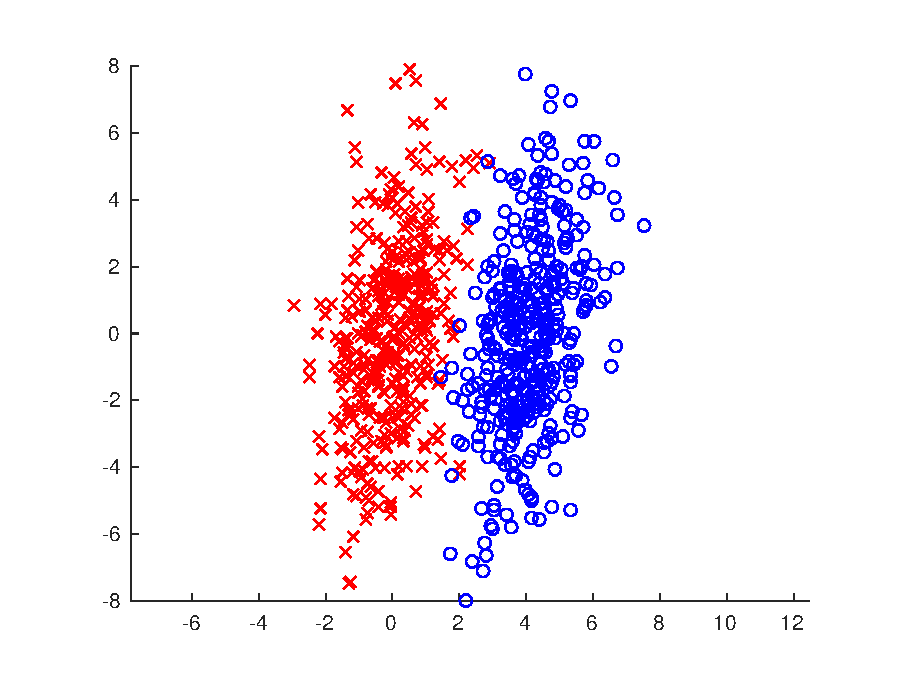
\includegraphics[width=0.5\textwidth]{./matlab/hw1_7_1.eps}
\end{center}
\item
\begin{verbatim}
figure
hold on;

mu1=[0;0];
sigma1=[1 1 ; 1 8];
r1=chol(sigma1);
x1=repmat(mu1,1,400)+r1'*randn(2,400);

mu2=[4;0];
sigma2=[1 1 ; 1 8];
r2=chol(sigma2);
x2=repmat(mu2,1,400)+r2'*randn(2,400);

plot(x1(1,:),x1(2,:),'rx',x2(1,:),x2(2,:),'bo');
axis([-6 10 -8 8]);
axis equal;

hold off;
\end{verbatim}
\end{itemize}

\newpage

\item ~\\
\begin{equation}
\nonumber
x_1 \sim \mathcal{N} \left(\left[\begin{array}{c}
0 \\
0 \\
\end{array}\right], \left[\begin{array}{cc}
1 & 1 \\
1 & 8 \\
\end{array}\right] \right),~
x_2 \sim \mathcal{N} \left(\left[\begin{array}{c}
4 \\
0 \\
\end{array}\right], \left[\begin{array}{cc}
2 & 0 \\
0 & 2 \\
\end{array}\right]\right)
\end{equation}
\end{enumerate}

\begin{itemize}
\item ~\\
\begin{center}
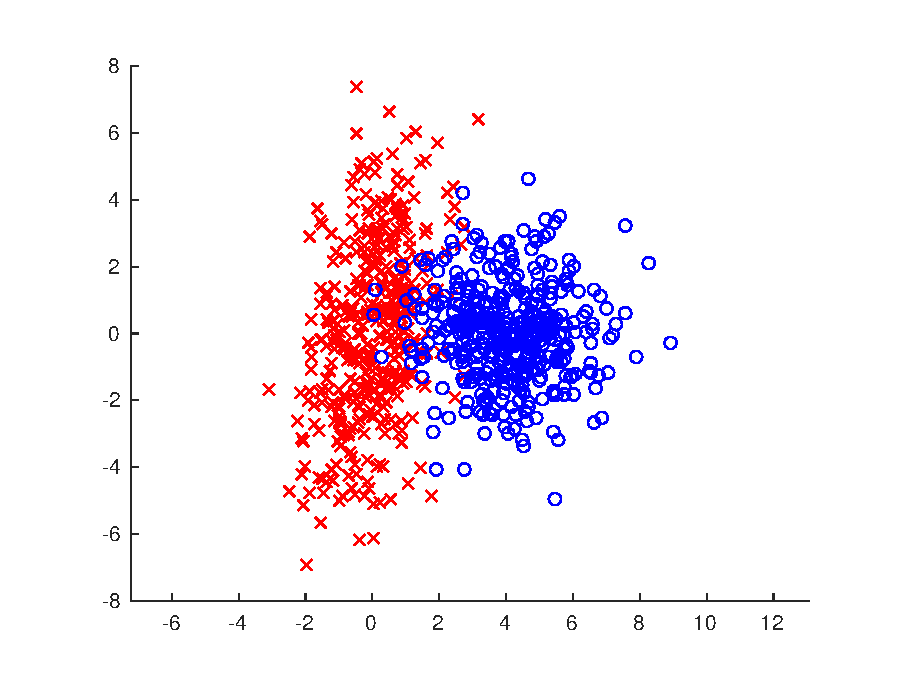
\includegraphics[width=0.5\textwidth]{./matlab/hw1_7_2.eps}
\end{center}
\item
\begin{verbatim}
figure
hold on;

mu1=[0;0];
sigma1=[1 1 ; 1 8];
r1=chol(sigma1);
x1=repmat(mu1,1,400)+r1'*randn(2,400);

mu2=[4;0];
sigma2=[2 0 ; 0 2];
r2=chol(sigma2);
x2=repmat(mu2,1,400)+r2'*randn(2,400);

plot(x1(1,:),x1(2,:),'rx',x2(1,:),x2(2,:),'bo');
axis([-6 10 -8 8]);
axis equal;

hold off;
\end{verbatim}
\end{itemize}

\newpage

\section*{Problem 8}

A two-dimensional feature vector is use to select one of two classes shown in
Figure 1. The joint PDFs are uniform over a square for class $\omega_1$ and a triangle
for class $\omega_2$. For each case, determine the probability of assigning $x$ to the wrong
class $\omega$ (compute $\epsilon_1$ and $\epsilon_2$), and the total probability of error (compute $P_e$).

\begin{center}
\includegraphics[width=0.7\textwidth]{./img/P8.png}
\end{center}

\begin{enumerate}
\item Case 1: $P(\omega_1)=P(\omega_2)$\\
\textbf{Answer:}\\
Define the square as $A$, and the triangle as $B$\\
Then the area of $A$, $S(A)=16$, and the area of $B$, $S(B)=16$.
$$\left\{\begin{array}{rcl}
f(\vec{x}|\omega_1) & = & \left\{\begin{array}{cc}
\frac{1}{16} & \vec{x} \in A\\
0 & \vec{x} \not \in A\\
\end{array}\right. \\
f(\vec{x}|\omega_2) & = & \left\{\begin{array}{cc}
\frac{1}{16} & \vec{x} \in B\\
0 & \vec{x} \not \in B\\
\end{array}\right. \\
\end{array}\right.$$

$$\left\{\begin{array}{rcl}
\epsilon_1 & = & f(\vec{x}|\omega_1)S(B-A)=\frac{1}{16}*8=1/2 \\
\epsilon_2 & = & f(\vec{x}|\omega_2)S(A-B)=\frac{1}{16}*8=1/2 \\
\end{array}\\
\right.$$

$$P_e=\epsilon_1 P(\omega_1)+\epsilon_2 P(\omega_2)=P(\omega_2)$$
\item Case 2: $P(\omega_1)=2P(\omega_2)$\\
\textbf{Answer:}

$$\left\{\begin{array}{rcl}
\epsilon_1 & = & f(\vec{x}|\omega_1)S(B-A)=\frac{1}{16}*8=1/2 \\
\epsilon_2 & = & f(\vec{x}|\omega_2)S(A-B)=\frac{1}{16}*8=1/2 \\
\end{array}\\
\right.$$

$$P_e=\epsilon_1 P(\omega_1)+\epsilon_2 P(\omega_2)=\frac{3}{2}P(\omega_2)$$

\end{enumerate}

\newpage

\section*{Problem 8}

\begin{enumerate}
	\item Write the name(s) of your project partner(s). Teams of 2 or 3 people.\\
	\textbf{Answer:} Iljoo Baek, Mengwen He (Alex)
	\item Describe in a few sentences, two ideas of possible projects that you want to pursue.\\
	\textbf{Answer:}
	\begin{enumerate}
		\item Use camera to detect road lane marks on a road. 
		\item Track the vehicle's lane change behavior from the camera. (Main goal)
		\item Combine the low-precise GPS/IMU and concise digital map to decrease the global localization error. (Additional goal)
	\end{enumerate}
\end{enumerate}

\end{document}

